% Created 2018-08-27 Mon 11:46
% Intended LaTeX compiler: pdflatex

\documentclass[12pt,a4paper]{article}
\def\pgfsysdriver{pgfsys-dvipdfm.def}

\usepackage{fontspec,indentfirst}
\usepackage{xunicode}% provides unicode character macros
\usepackage{xltxtra} % provides some fixes/extras
\usepackage[margin=1.5cm]{geometry}
\usepackage{tikz}

\XeTeXlinebreaklocale "zh"
\XeTeXlinebreakskip = 0pt plus 1pt minus 0.1pt


\newfontfamily\xingkai{"NSimSun"}
\newfontfamily\caiyun{"NSimSun"}
\newfontfamily\kai{"NSimSun"}
\newfontfamily\fs{"NSimSun"}
\newfontfamily\li{"NSimSun"}
\newfontfamily\xinwei{"NSimSun"}
\newfontfamily\yao{"NSimSun"}
\newfontfamily\hei{"NSimSun"}
\newfontfamily\song{"NSimSun"}

\setmainfont{"NSimSun"}

\renewcommand{\baselinestretch}{1.2}

% [FIXME] ox-latex 的設計不良導致 hypersetup 必須在這裡插入
\usepackage{hyperref}
\hypersetup{
  colorlinks=true, %把紅框框移掉改用字體顏色不同來顯示連結
  linkcolor=[rgb]{0,0.37,0.53},
  citecolor=[rgb]{0,0.47,0.68},
  filecolor=[rgb]{0,0.37,0.53},
  urlcolor=[rgb]{0,0.37,0.53},
  pagebackref=true,
  linktoc=all,}
\author{贵州理工学院 大数据学院 张森}
\date{\today}
\title{在Windows上安装miniconda}
\begin{document}

\maketitle
\tableofcontents

Miniconda 是 Anaconda 的精简发行版。Anaconda本身分为 Anaconda 2 和
Anaconda 3 系列,分别提供对 python 2.x 语言 和 python 3.x 语言的支持。
本门课使用 Anaconda 3(Miniconda 3)以及相关的工具库进行网络数据包分析
工具。

\section{下载 Miniconda3}
\label{sec:org9b7b77f}

从 \url{https://mirrors.tuna.tsinghua.edu.cn/anaconda/miniconda/} 下载
Miniconda3 。依据你的操作系统是64位还是32位的Windows,下载对应的版本。
如果操作系统是64位的Windows,下载
\url{https://mirrors.tuna.tsinghua.edu.cn/anaconda/miniconda/Miniconda3-latest-Windows-x86\_64.exe};
如果操作系统是32位的Windows,下载
\url{https://mirrors.tuna.tsinghua.edu.cn/anaconda/miniconda/Miniconda3-latest-Windows-x86.exe}。

下面的命令会以在64位Windows上安装
\texttt{Miniconda3-latest-Windows-x86\_64.exe} 为例。在32位的情况下,请对命令
里的参数作相应替换。

当然,也可以选择安装完整版的Anaconda3。完整版的Anaconda3从
\url{https://mirrors.tuna.tsinghua.edu.cn/anaconda/archive/} 下载。相应地,
需要替换后续命令里的部分参数。

\section{安装 Miniconda 3}
\label{sec:orgb61dbbd}

当然,可以双击 \texttt{Miniconda3-latest-Windows-x86\_64.exe} 直接安装,所有
配置选项采用默认设置。也可以用下面的方法安装。

\subsection{静默安装  Miniconda 3}
\label{sec:org51065c6}

把下列命令复制到记事本(或者你钟爱的编辑器)里,另存为
\texttt{Miniconda3-latest-Windows-x86\_64.exe} 所在的目录里的
\texttt{install\_miniconda3.bat} 文件。

\begin{verbatim}
start /wait ""  Miniconda3-latest-Windows-x86_64.exe /InstallationType=JustMe /RegisterPython=0 /S /D=%UserProfile%\Miniconda3
\end{verbatim}

然后双击 \texttt{install\_miniconda3.bat} ,等待执行完成,Miniconda3 会被安装在
\texttt{\%UserProfile\%\textbackslash{}Miniconda3} (默认情况下,会在 \texttt{C:\textbackslash{}Users\textbackslash{}<你的用户名>\textbackslash{}Miniconda3} )目录里。

\section{设置python软件包更新源的镜像}
\label{sec:org4926427}

用文本编辑器(比如notepad)编辑 \%APPDATA\%\pip\pip.ini 文件,在里面顶
格输入下面三行配置并保存(请务必注意配置文件的后缀名,必须是.ini,不
能是.ini.txt或者.txt):

\begin{verbatim}
[global]
trusted-host=pypi.tuna.tsinghua.edu.cn
index-url=https://pypi.tuna.tsinghua.edu.cn/simple
\end{verbatim}

采用国内的python软件包更新源镜像,通常会提升软件包的下载速率。

\section{设置Anaconda的源}
\label{sec:org3bb241c}

同样地,也是为了后续使用conda命令时能够比较快地下载软件包,在开始菜
单里找到 \texttt{Anaconda3} ,点击 \texttt{Anaconda Prompt} ,然后在出来的cmd命令
行窗口里输入下列命令并回车:

\begin{verbatim}
conda config --add channels 'https://mirrors.tuna.tsinghua.edu.cn/anaconda/pkgs/free/'
conda config --set show_channel_urls yes
# 看看当前的 config 是什么样的
conda config --show  
\end{verbatim}

好了,这样可以开心的下载东西了。

\subsection{如何删除添加的源呢?}
\label{sec:orgb0ade4d}

这一步Just for your information,目前没有必要执行。

\begin{verbatim}
conda config --remove channels 'https://mirrors.tuna.tsinghua.edu.cn/anaconda/pkgs/free/' 
\end{verbatim}

\section{更新pip}
\label{sec:orgeec1633}

在开始菜单里找到 \texttt{Anaconda3} ,点击 \texttt{Anaconda Prompt} ,然后在出来的
cmd命令行窗口里输入下列命令并回车:

\begin{verbatim}
python -m pip install -U pip
\end{verbatim}

\begin{figure}[htbp]
\centering
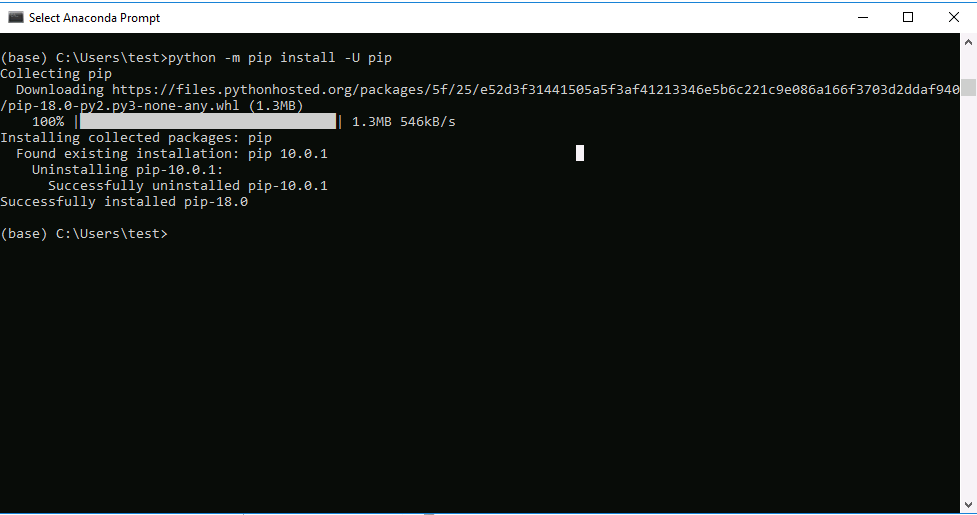
\includegraphics[width=.9\linewidth]{./images/chap0/update_pip.png}
\caption{\label{fig:org5de5729}
更新pip}
\end{figure}

注意看cmd命令行窗口是否输出了红色和黄色的错误和警告信息。如果有,则
表明用pip安装/更新软件包出错(下同)。

\section{安装分析wireshark数据包文件所需的工具库}
\label{sec:org92e9036}

在开始菜单里找到 \texttt{Anaconda3} ,点击 \texttt{Anaconda Prompt} ,然后在出来的
cmd命令行窗口里输入下列命令并回车:

\begin{verbatim}
pip install pyshark spyder jupyter
\end{verbatim}

不出意外的话会看到:

\begin{figure}[htbp]
\centering
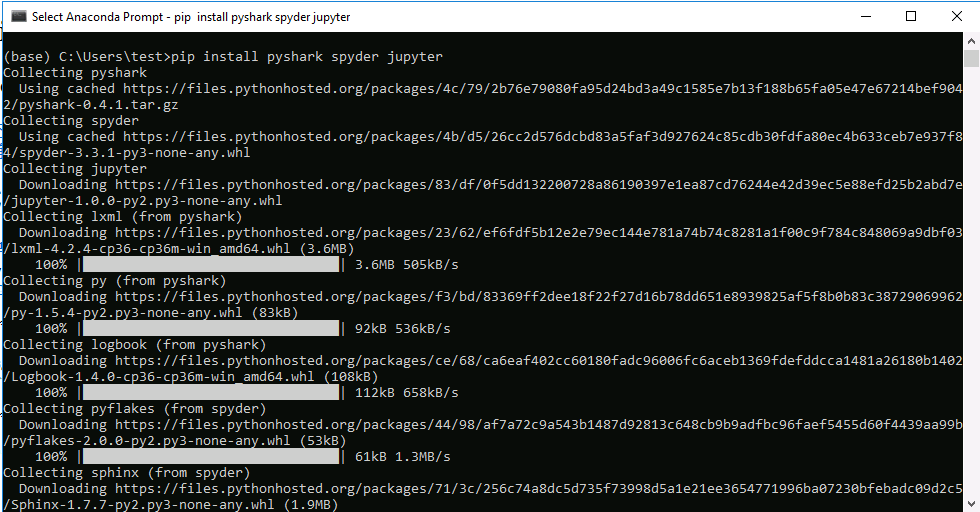
\includegraphics[width=.9\linewidth]{./images/chap0/install_pyshark_spyder_jupyter.png}
\caption{\label{fig:orgc1166ac}
安装分析wireshark数据包文件所需工具库}
\end{figure}
\end{document}